\documentclass[letterpaper,11pt]{article}

\author{Jacob Thomas Errington}
\date{5 November 2015}
\title{Assignment \#4\\Theory of Computing -- COMP 330}

\usepackage{amsmath,amssymb,amsthm}
\usepackage{qtree}

\usepackage[margin=2.0cm]{geometry}

\usepackage{tikz}
\usetikzlibrary{automata}

\newtheorem{proposition}{Proposition}

\begin{document}

\maketitle

\begin{enumerate}
    \item Let $\#_x(s)$ represent the number of occurrences of the letter $x$
        in the string $s$.

        \begin{proposition}
            The given grammar generates the set of all strings $w \in \Sigma^*$
            such that $\#_a(w) = \#_b(w)$.
        \end{proposition}

        \begin{proof}
            Suppose we have a string having an equal number of occurrences of
            $a$s and $b$s. Of course, somewhere in this string, we will
            encounter the substring $ab$ or $ba$, which we will replace with an
            $S$, as this matches a rule in the grammar. Then, we may replace
            this $S$ with $\epsilon$, since that is a possible string generated
            by $S$. This procedure effectively reduces the length of the given
            string by $2$ on each iteration, and furthermore preserves the
            invariant that the string have equal occurrences of $a$ and $b$.
            Because the length is strictly decreasing, we arrive at the empty
            string, concluding that the string is recognized by the grammar.

            Now to show that the given grammar generates all strings of having
            equal occurrences of $a$ and $b$, we will use a form of induction.
            Of course, $\epsilon$ has equal occurrences of $a$ and $b$, and is
            a possible production of $S$. Now suppose $s$ and $s^\prime$ have
            equal occurrences of $a$ and $b$. Then, $asb$ and $bsa$ have equal
            occurrences of $a$ and $b$ since in each case, one of each letter
            is added. Also, $ss^\prime$ has equal occurrences of $a$ and $b$
            since $\#_a(s) + \#_a(s^\prime) = \#_a(ss^\prime)$ and
            $\#_b(s) + \#_b(s^\prime) = \#_b(ss^\prime)$.
        \end{proof}

    \item
        To show that the language for simple C-style expressions is ambiguous,
        we will present a string having multiple valid parses.

        We will consider the string $a+++b$, and show that there is more than
        one possible parse for it, as seen in the parse trees in figures
        \ref{fig:postincrement} and \ref{fig:preincrement}.

        \begin{figure}
            \Tree
            [.S
                [.V
                    [.Post
                        [.I
                            $a$
                        ]
                        $+$
                        $+$
                    ]
                ]
                $+$
                [.V
                    [.I
                        $b$
                    ]
                ]
            ]

            \caption{
                A parse tree for the postincrement interpretation of $a+++b$.
            }
            \label{fig:postincrement}
        \end{figure}

        \begin{figure}
            \Tree
            [.S
                [.V
                    [.I
                        $a$
                    ]
                ]
                $+$
                [.V
                    [.Pre
                        [.I
                            $b$
                        ]
                        $+$
                        $+$
                    ]
                ]
            ]

            \caption{
                A parse tree for the preincrement interpretation of $a+++b$.
            }
            \label{fig:preincrement}
        \end{figure}

        Since the given grammar is not recursive, the unary incrementing
        operators cannot be nested; the only ambiguous string is
        $a+++b$. We can write unambiguous grammars for each interpretation by
        exhausting all the possible parses, of which there are only finitely
        many due to the lack of recursion, and then eliminating common
        subexpressions of rules by introducing new rules for them. We have used
        that procedure in the following two unambiguous grammars.

        First, here is a grammar that will parse $a+++b$ as including a
        post-increment.
        \begin{align*}
            S &\to (I | \langle Pre \rangle) + (I | P ) \\
            S &\to \langle Post \rangle + P \\
            P &\to \langle Pre \rangle | \langle Post \rangle
        \end{align*}

        Next, we will write a grammar to parse $a+++b$ as including a
        pre-increment.
        \begin{align*}
            S &\to I + ( I | \langle Post \rangle ) \\
            S &\to P + (I | P) \\
            P &\to \langle Pre \rangle | \langle Post \rangle
        \end{align*}

        The $I$, $\langle Pre \rangle$, and $\langle Post \rangle$ productions
        are exactly as in the original grammar.

    \item
        Here is a Chomsky Normal Form grammar for the language of matched
        brackets with two kinds of brackets.
        \begin{align*}
            S &\to \epsilon \\
            S &\to AS \\
            A &\to P_1 Q_1 \\
            P_1 &\to P_1^\prime S \\
            P_1^\prime &\to ( \\
            Q_1 &\to ) \\
            A &\to P_2 Q_2 \\
            P_2 &\to P_2^\prime S \\
            P_2^\prime &\to [ \\
            Q_2 &\to ] \\
        \end{align*}

    \item Figure \ref{fig:pda} shows a pushdown automaton for the grammar given
        in the previous answer.

        \begin{figure}
            \centering

            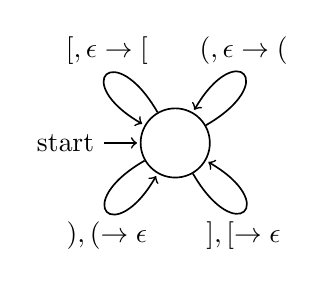
\begin{tikzpicture}[
                    ->,
                    shorten >=1pt,
                    auto,
                    node distance=2.8cm,
                    semithick,
                    looseness=12
                ]
                \tikzstyle{every state}=[
                    fill=white,
                    draw=black,
                    text=black
                ]

                \node[initial, state] (A) {} ;

                \path
                (A) edge [out=30, in=60]
                    node [above]
                    {$(,\epsilon \to ($}
                    (A)
                (A) edge [out=120, in=150]
                    node [above]
                    {$[,\epsilon \to [$}
                    (A)
                (A) edge [out=210, in=240]
                    node [below]
                    {$),( \to \epsilon$}
                    (A)
                (A) edge [out=300, in=330]
                    node [below]
                    {$],[ \to \epsilon$}
                    (A)
                ;
            \end{tikzpicture}

            \caption{
                A pushdown automaton for recognizing the language of balanced
                braces with two types of braces.
            }

            \label{fig:pda}
        \end{figure}

    \item
        The following is a grammar for the language
        $\{a^n b^m c^p | n \leq p \lor m \leq p\}$.
        \begin{align*}
            S &\to A_1 \\
            S &\to A_2 B_2 \\
            A_1 &\to a A C | B \\
            B_1 &\to \epsilon | b B \\
            C_1 &\to c | c C \\
            A_2 &\to \epsilon | a A_2 \\
            B_2 &\to \epsilon | b B_2 C_2 \\
            C_2 &\to c | c C_2
        \end{align*}

        Our strategy for building this grammar was to recognize that
        context-free languages are closed under union. Indeed, this grammar is
        built as the union of the two important cases, as the productions for
        $S$.

        The first group of productions is made to recognize the case where
        $\#_a \leq \#_c$, by placing one $C$ for each $a$, and inserting the
        $B$ production between the group of $a$s and the group of $C$s. Thus,
        we can have an arbitrary number of $b$s while ensuring that the number
        of $a$s is at most the number of $c$s.

        The second group of productions is made to recognize the case where
        $\#_b \leq \#_c$, by producing arbitrarily many $a$s and then producing
        an equal number of $b$s and $C$s. Each $C$ in turn can expand to
        arbitrarily many $c$s, but this ensures that there are at most as many
        $b$s as $c$s.

    \item
        Consider the language
        $L = \{a^n b^m c^p | (n \leq p \lor m \leq p), n > 0, m > 0, p > 0\}$.
        We notice that
        $\min{(L)} = \{a^n b^m c^p | p = \min{(n, m)}, n > 0, m > 0, p > 0\}$.
        Indeed, the most that this minimization process can conceptually do is
        remove extraneous occurrences of $c$ from the ends of strings.

        We will show that $\min{(L)}$ is not context-free, hence showing that
        the set of context-free languages is not closed under the $\min$
        operation. To do so, we will use the pumping lemma for context-free
        languages.

        \begin{proposition}
            The set of context-free languages is not closed under the $\min$
            operation.
        \end{proposition}

        \begin{proof}
            By the pumping lemma for context-free languages.

            Demon picks $p$.

            I pick $s = a^{p+1} b^{p+1} c^{p+1}$. Clearly, $s \in \min{(L)}$
            since $p+1 = \min{(p+1, p+1)}$.

            Demon picks $u,v,w,x,y \in \Sigma^*$ such that $s = uvwxy$ and
            $|vx| > 0$ and $|vwx| \leq p$.

            Our choice of $i$ will depend on the split chosen by the demon;
            we will analyze the possible splits chosen by the demon to show
            that our choice of $i$ will always result in a string not in the
            language.

            If the demon chooses both $v$ and $x$ to both lie within the region
            of $a$s or the region of $b$s, then we can pick $i = 0$. This will
            reduce the number of letters in that region by at least $1$,
            resulting in a new minimum not matched by the number of $c$s,
            so the resulting string is not in the language.

            If the demon chooses both $v$ and $x$ to both lie in the region
            of $c$s, then we can pick $i = 2$, making the number of $c$s
            greater than the minimum, which results in a string not in the
            language.

            For all the following cases, we can pick $i = 2$.

            If the demon chooses $v$ or $x$ to straddle the boundary between
            two different letters, then pumping up will result in an
            alternation of letters. We thus need not concern ourselves with
            those cases.

            If the demon chooses $v$ in the region of $a$s and $x$ in the
            region of $b$s, then the number of $c$s will be less than the
            number of $a$s and the number of $b$s. Hence the resulting string
            is not in the language.

            If the demon chooses $v$ in the region of $a$s and $x$ in the
            region of $c$s, then we have $a^{4p} b^{p+1} c^{2p+2}$ and
            $2p+2 > p + 1$. The resulting string is thus not in the language.

            Finally, if the demon chooses $v$ in the region of $b$s and $x$ in
            the region of $c$s, then we have $a^{2p} b^{2p + 2} c^{2p + 2}$ and
            $2p + 2 > 2p$. The resulting string is thus not in the language.

            Hence, $\min{(L)}$ is not context-free, and the set of context-free
            languages is not closed under the $\min$ operation.
        \end{proof}

\end{enumerate}

\end{document}
